%------------------------------------------------------------
% Meeting with Bernhardt - 7/11/23
% E. Hazen - Boston University
%------------------------------------------------------------

\pdfminorversion=4   % fix Acrobat error
\documentclass{beamer}
\usepackage{graphicx}
\usepackage{tikz}    % for logo only
\usepackage{xcolor}
\usepackage[absolute,overlay]{textpos}
\usepackage{makecell}
\usepackage{array}
\usepackage{siunitx}

% hyperref should always be the last one, except with glossaries
\usepackage{hyperref}

\definecolor{my-red}{RGB}{128,0,0}
\definecolor{my-green}{RGB}{0,96,0}
\definecolor{my-blue}{RGB}{0,0,128}
\definecolor{my-orange}{RGB}{160,83,0}
\definecolor{my-violet}{RGB}{142,0,209}
\definecolor{my-aqua}{RGB}{0,96,96}
\definecolor{my-olive}{RGB}{89,124,0}

\newcommand{\tred}[1]{\textcolor{my-red}{#1}}
\newcommand{\tgreen}[1]{\textcolor{my-green}{#1}}
\newcommand{\tblue}[1]{\textcolor{my-blue}{#1}}
\newcommand{\torange}[1]{\textcolor{my-orange}{#1}}
\newcommand{\tviolet}[1]{\textcolor{my-violet}{#1}}
\newcommand{\taqua}[1]{\textcolor{my-aqua}{#1}}
\newcommand{\tolive}[1]{\textcolor{my-olive}{#1}}

\hypersetup{
  colorlinks = true,
}

\begin{document}

% Add footer text
\addtobeamertemplate{footline}{
  \parbox{\linewidth}{\vspace*{-8pt}
    ~~~ Slide \insertframenumber/\inserttotalframenumber
    ~~~ 2023-07-11 ~~~
    E.~Hazen}
}

% Move footnotes above footline
\addtobeamertemplate{footnote}{}{\vspace{0.1in}}

% add BU + ATLAS logo
\addtobeamertemplate{frametitle}{}{%
\begin{tikzpicture}[remember picture,overlay]
\node[anchor=north east,yshift=2pt] at (current page.north east)
{
\includegraphics[height=0.8cm]{figs/BU_NPC.png}};
\end{tikzpicture}}

\newcommand{\spage}[1]{
\begin{frame}
  \begin{tikzpicture}[remember picture, overlay]
  \node[anchor=north]at(current page.north){
     \includegraphics[width=0.95\paperwidth]{#1}
  };
  \end{tikzpicture}
\end{frame}
}


\begin{frame}
        
\frametitle{Optode Readout}

  \begin{columns}[T]
  \column{0.7\textwidth}

  Specification
  \begin{itemize}
  \scriptsize
  \item Low-noise transimpedance gain = ??
  \item Separate LDO for each channel +5V
  \item Fit in Hammond 1551QGY box
  \end{itemize}

  \column{0.4\textwidth}

  \vskip -0.2in
  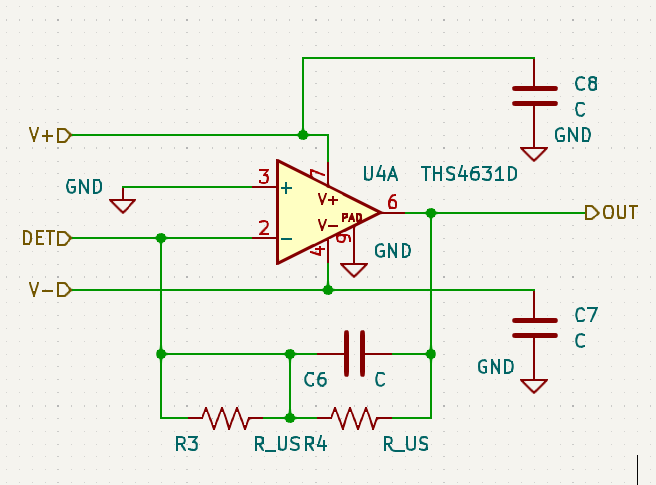
\includegraphics[width=\textwidth]{figs/schem-amp.png}
  \vskip 0.2in
  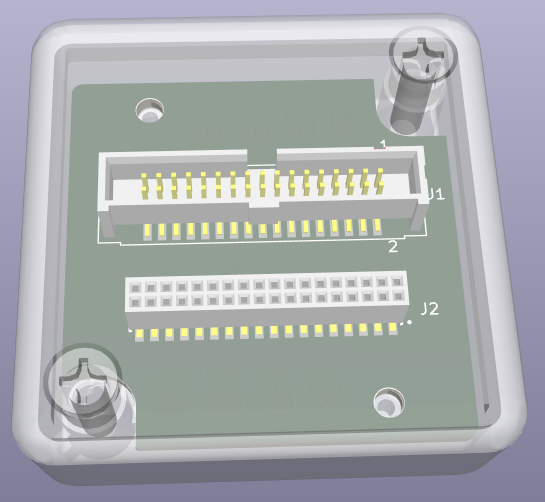
\includegraphics[width=\textwidth]{figs/3D-pre-top.png}

  \end{columns}
  
\end{frame}




\begin{frame}
  \frametitle{OP-Amp Choice}

  \begin{columns}
  \column{0.4\textwidth}
  \scriptsize
  Tentative op-amp choice:  THS4631
    \begin{itemize}
    \scriptsize
    \item Low noise
    \item Small package
    \item 30V power supply max
    \item Availability
    \end{itemize}
  \column{0.6\textwidth}

  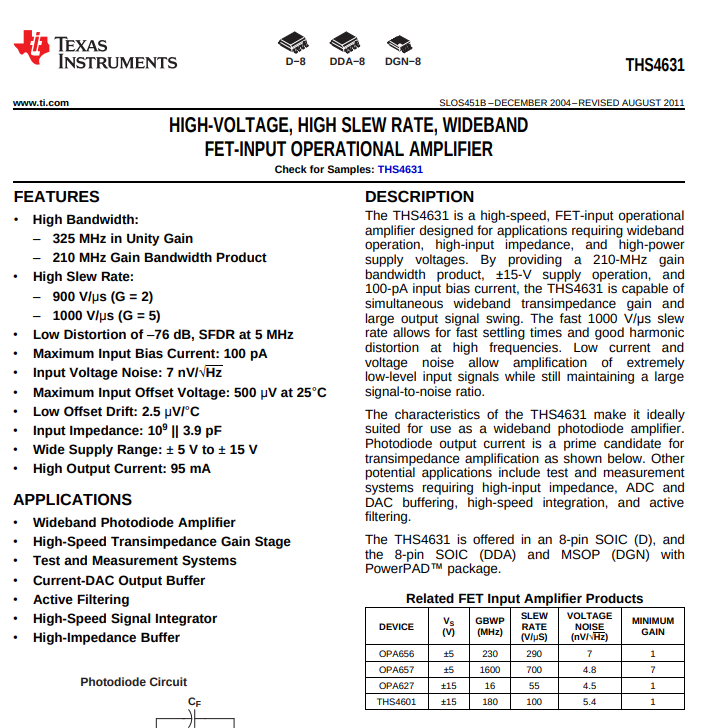
\includegraphics[width=\textwidth]{figs/ths4631-data.png}

  \end{columns}






  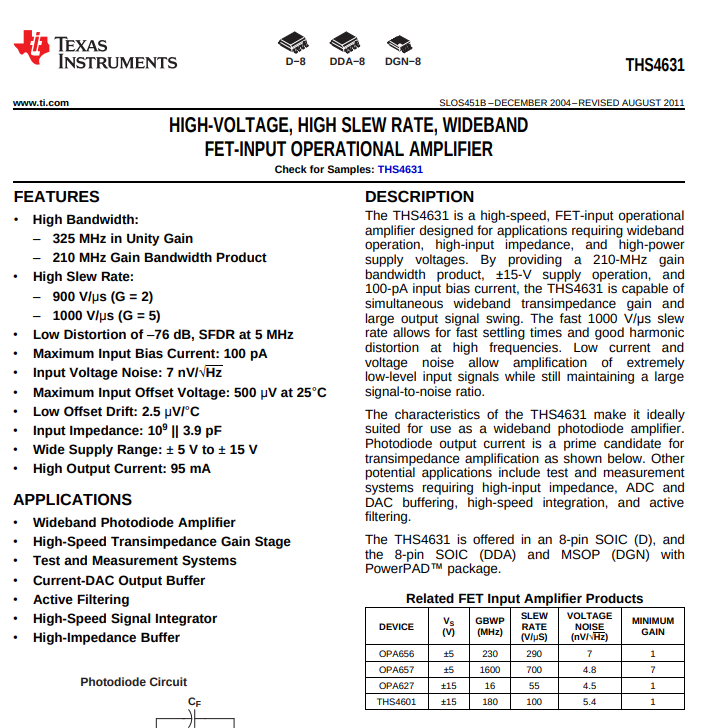
\includegraphics[width=\textwidth]{figs/ths4631-data.png}

\end{frame}



%% \title{ATCA Overview in LHC}
%% \author
%% {E.~Hazen {\em on behalf of many LHC collaborators}}
%% 
%% \begin{frame}
%%   \includegraphics[width=\textwidth]{figs/lhc-web.png}
%%   \vskip 0.3in
%%   \begin{centering}
%%   Summary of ATCA use in LHC \\
%%   (with emphasis on SoM) \\
%%   {\em E. Hazen, Boston University} \\
%%   \end{centering}
%% \end{frame}
%% 
%% \begin{frame}
%%   \frametitle{The Large Hadron Collider}
%%   \framesubtitle{Located outside Geneva, Switzerland -- Four Experiments}
%%   \begin{columns}
%%   \column{0.25\textwidth}
%%     \includegraphics[width=\textwidth]{figs/atlas.jpg} \\
%%     ATLAS
%%   \column{0.25\textwidth}
%%     \includegraphics[width=\textwidth]{figs/cms.jpg} \\
%%     CMS
%%   \column{0.25\textwidth}
%%     \includegraphics[width=\textwidth]{figs/alice.jpg} \\
%%     ALICE
%%   \column{0.25\textwidth}
%%     \includegraphics[width=\textwidth]{figs/lhcb.jpg} \\
%%     LHCb
%%   \end{columns}
%%   \vskip 0.3in
%%   The Boston University EDF has built readout electronics
%%   for many parts of the ATLAS and CMS experiments, and consulted
%%   on systems for the others.
%% \end{frame}
%% 
%% 
%% \begin{frame}
%% \frametitle{ATCA Blades in LHC}
%% \framesubtitle{Installed starting in 2026}
%% 
%%   \begin{columns}
%%   \column{0.5\textwidth}
%%     \includegraphics[width=\textwidth]{figs/MDTTP-demonstrator-photo-labeled}
%% 
%%     \tiny
%%     \tblue{{\em e.g.} ATLAS L0MDT trigger processor demonstrator \\
%%       (designed by BU and MPI - Germany)}
%%   \column{0.5\textwidth}
%% 
%%   \begin{itemize}
%%   \item ATLAS:  total about 1450 blades in 120 shelves
%%   \item CMS:    total about 1200 blades in 150 shelves
%%   \end{itemize}
%% 
%%   \end{columns}
%%   
%% 
%% 
%% 
%% \end{frame}
%% 
%% \begin{frame}
%%   \frametitle{ATCA Blades in CMS}
%% 
%%     \begin{columns}
%%     \column{0.9\textwidth}
%% 
%%     \vskip -0.5in
%%     \begin{itemize}
%%     \item Serenity Family (European institutes) \\
%%       {\tiny Bristol University, Imperial College, Ioannina, INFN, KIT, RAL, SACLAY, TIFR}
%%       \begin{itemize}
%%       \scriptsize
%%       \item Demonstrator uses COM-Express Type 10 (Atom)
%%       \end{itemize}
%%       \vskip 0.15in
%%     \item APOLLO Family (US institutes) \\
%%       {\tiny Cornell, Boston University, UMass, UCI, Colorado, Northwestern}
%%       \begin{itemize}
%%       \scriptsize
%%       \item Demonstrator uses Enclustra Mercury ZX1
%%       \end{itemize}
%%       \vskip 0.15in
%%     \item APx Family (US institutes) \\
%%       {\tiny Virginia, Fermilab, Wisconsin, U-Florida, UI Chicago, Notre Dame}
%%       \begin{itemize}
%%       \scriptsize
%%       \item Demonstrator uses in-house ELM1 board (Zynq 7-series)
%%       \end{itemize}
%% 
%%     
%%       \vskip 0.15in
%%       \tblue{Total $\approx 1200$ blades of perhaps 20 different types.}
%% 
%% 
%%     \end{itemize}
%%             
%%     \column{0.15\textwidth}
%% 
%%     \includegraphics[width=\textwidth]{figs/serenity-sm.jpg}
%%     \vskip 0.3in
%%     \includegraphics[width=\textwidth]{figs/apollo-sm.jpg}
%%     \vskip 0.3in
%%     \includegraphics[width=\textwidth]{figs/apx-sm.jpg}
%% 
%%     \end{columns}
%%         
%% \end{frame}
%% 
%% \begin{frame}
%%   \frametitle{APOLLO Blade Family}
%%   \framesubtitle{Typical configuration as an example}
%%   \vskip -0.3in
%%   \begin{columns}
%%   \column{0.7\textwidth}
%%   \includegraphics[width=\textwidth]{figs/I2C_Fig.pdf}  
%%   \column{0.4\textwidth}
%%     \scriptsize
%%     SoM Functions
%%     \begin{itemize}
%%     \item Ethernet interface
%%     \item I2C device access/control
%%     \item AXI chip-to-chip
%%     \item UART interfaces
%%     \end{itemize}
%%     
%% 
%% 
%%   \end{columns}
%% \end{frame}
%% 
%% 
%% 
%% 
%% \begin{frame}
%%   \frametitle{SoM Use in LHC Upgrades}
%% 
%%   Most (all?) LHC ATCA blades will use an SoM for:
%%     \begin{itemize}
%%     \scriptsize 
%%     \item Configuration, control, monitoring
%%     \item Hardware control of clock, power, optical modules, FPGA configuration
%%     \item Run control of processing FPGAs:  read/write status/control registers
%%     and memories/LUTs, read counters, histograms
%%     \end{itemize}
%% 
%%   \vskip 0.2in
%%   
%%   General Requirements:
%%     \begin{itemize}
%%     \scriptsize
%%     \item 64-bit ARM, dual or quad core
%%     \item $\ge $4GB main memory
%%     \item eMMC or QSPI flash
%%     \item uSD card interface (remote front panel mount)
%%     \item 2x gigabit Ethernet
%%     \item Minimum of 4 transceivers capable of 10~Gbps
%%     \item Around 100-150 GPIOs exposed, with many routed
%%       as differential pairs.
%%     \end{itemize}
%% \end{frame}
%% 
%% \begin{frame}
%%   \frametitle{SoM Use in LHC Upgrades}
%%   \framesubtitle{Additional requirements/thoughts}
%% 
%%   \begin{columns}
%%   \column{0.3\textwidth}
%%   \tiny Typical COTS offering \\
%%   \includegraphics[width=0.5\textwidth]{figs/mercury.jpg} \\
%%   \tiny Enclustra Mercury \\
%%   XC7Z045 / 64 x 54 mm
%%   \vskip 0.5in
%%   HEP community \\
%%   \includegraphics[width=0.6\textwidth]{figs/elm1.jpg} \\
%%   \tiny Wisconsin ELM1 \\
%%   XC7Z045 /   84 x 75 mm
%%   \column{0.7\textwidth}
%%   Here are some other desirable features:
%%   \begin{itemize}
%%   \scriptsize
%%   \item Small form factor (like Mercury, Kria)
%%   \item On-board power supplies from bulk 12V
%%   \item External VCCO inputs (optional on-board)
%%   \end{itemize}
%% 
%%   \vskip 0.2in
%%   Issues for discussion:
%%     \begin{itemize}
%%     \scriptsize
%%     \item Multiple-source; long-term availability
%%     \item Access to all design details \\
%%       (design files; source code; manufacturing data)
%%     \item Attractive price / delivery
%%     \end{itemize}
%% 
%%   \end{columns}
%% \end{frame}
%% 
%% \begin{frame}[shrink=5]
%% \frametitle{SoM - Kria Option}
%% 
%%   \begin{columns}
%%   \column{0.3\textwidth}
%%     \includegraphics[width=\textwidth]{figs/som-k26-main.png}
%%   \column{0.7\textwidth}
%%     Kria issues for discussion:
%%     \begin{itemize}
%%     \scriptsize
%%     \item \tgreen{Pros:}
%%       \begin{itemize}
%%       \scriptsize
%%       \item Meets requirements for most blades
%%       \item Price is very attractive
%%       \item It is available!
%%       \end{itemize}
%%         
%%     \item \tred{Concerns:}
%%       \begin{itemize}
%%       \scriptsize
%%       \item Is long-term availability assured?
%%       \item Closed design (others provide schematics)
%%       \end{itemize}
%%     \end{itemize}
%%   \end{columns}
%% 
%%   \vskip 0.2in
%%   \tblue{Current status here at BU:}
%% 
%%   \begin{itemize}
%%   \scriptsize
%%   \item APOLLO blades (representing 300+ installed) use Enclustra Mercury+
%%   \item We are developing an adapter which will allow us to test Kria
%%   \item We must decide no later than early 2023 on an option: \\
%%     1. Stay with Enclustra \\
%%     2. Change to Kria \\
%%     3. Develop something in-house, or other?
%%   \end{itemize}
%% 
%%   \tblue{Finally:} \\
%%   \scriptsize
%%   \tgreen{I have the ear of ATLAS and CMS experiments electronics management, and they
%%   are looking to me for guidance on how to proceed.  This represents about 3000
%%   total ATCA blades.}
%% 
%% \end{frame}

\end{document}
